\pagestyle{fancy}
\fancyhead{} % clear all header fields
\fancyhead[LO,CE]{Réalisation}
\fancyhead[RO,LE]{2024-2025}

\chapter{Réalisation du projet}
\section{Mise en place de l'environnement de développement}
\subsection{Configuration de Firebase Realtime Database}
Dans Firebase, tout est organisé en projets afin de pouvoir regrouper les ressources et de faciliter la gestion des règles et des politiques de sécurité. La première étape consiste donc à créer un projet dans Firebase, comme illustré sur la figure~\ref{fig:creation_projet_dans_firebase}.

\begin{figure}[H]
   \centering
   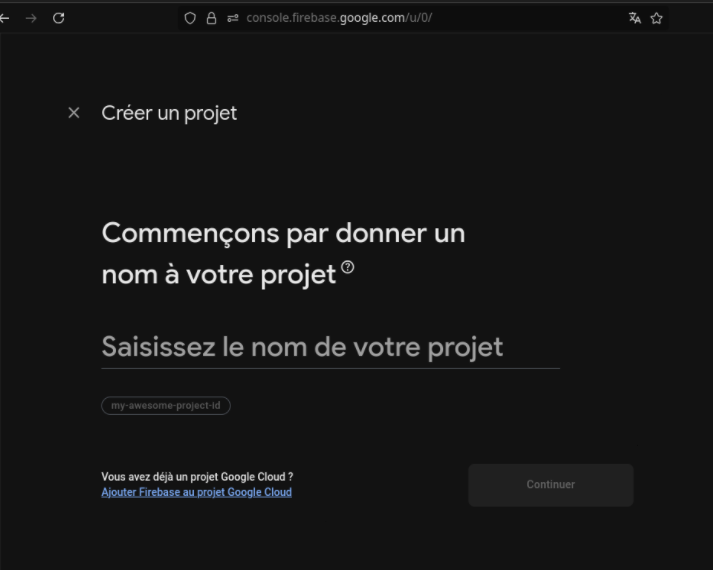
\includegraphics[scale=0.5]{firebase-project-setup.png}
   \caption{Création de projet dans Firebase}
   \label{fig:creation_projet_dans_firebase}
\end{figure}

Ensuite, on doit activer Firebase Authentication afin de pouvoir l'utiliser comme méthode d'authentification dans l'application mobile. Dans la console d'administration de Firebase, il faut aller dans \textbf{Créer > Authentication > Méthode de connexion > Ajouter un fournisseur > Adresse e-mail/Mot de passe}, puis activer la fonctionnalité comme illustré dans la figure~\ref{fig:activation_de_Firebase_Auth}.

\begin{figure}[H]
   \centering
   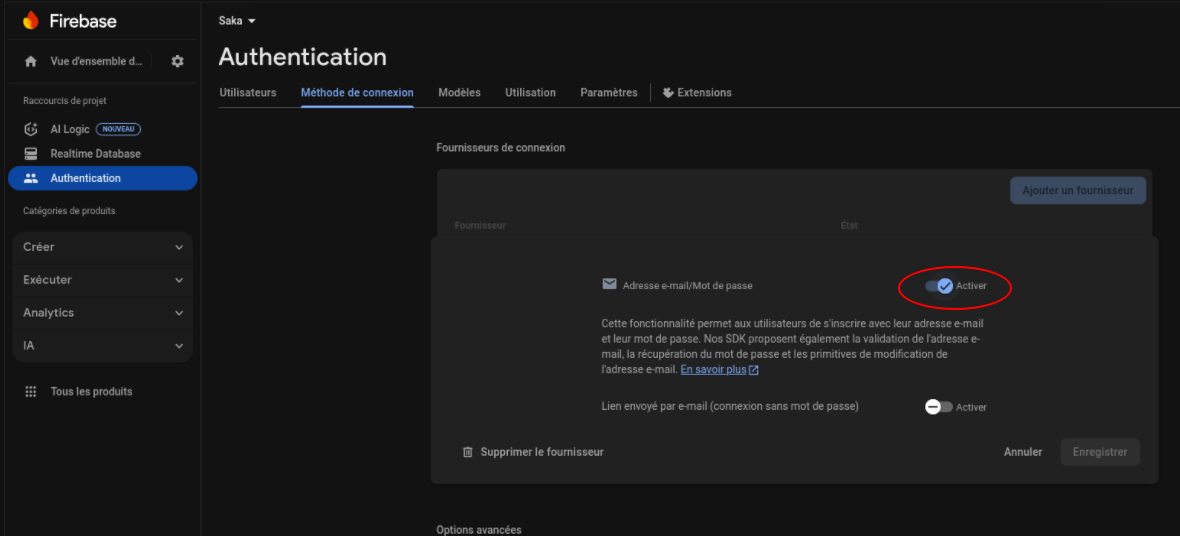
\includegraphics[scale=0.5]{firebase_auth.png}
   \caption{Activation de Firebase Authentication}
   \label{fig:activation_de_Firebase_Auth}
\end{figure}

Pour créer l'instance de Realtime Database, il faut passer par \textbf{Créer > Realtime Database > Créer une base de données}, puis suivre les étapes de réglage des options et des règles de sécurité. Une fois activée, on obtient un lien comme illustré sur la figure~\ref{fig:db_dans_realtime_db}. 

\begin{figure}[H]
   \centering
   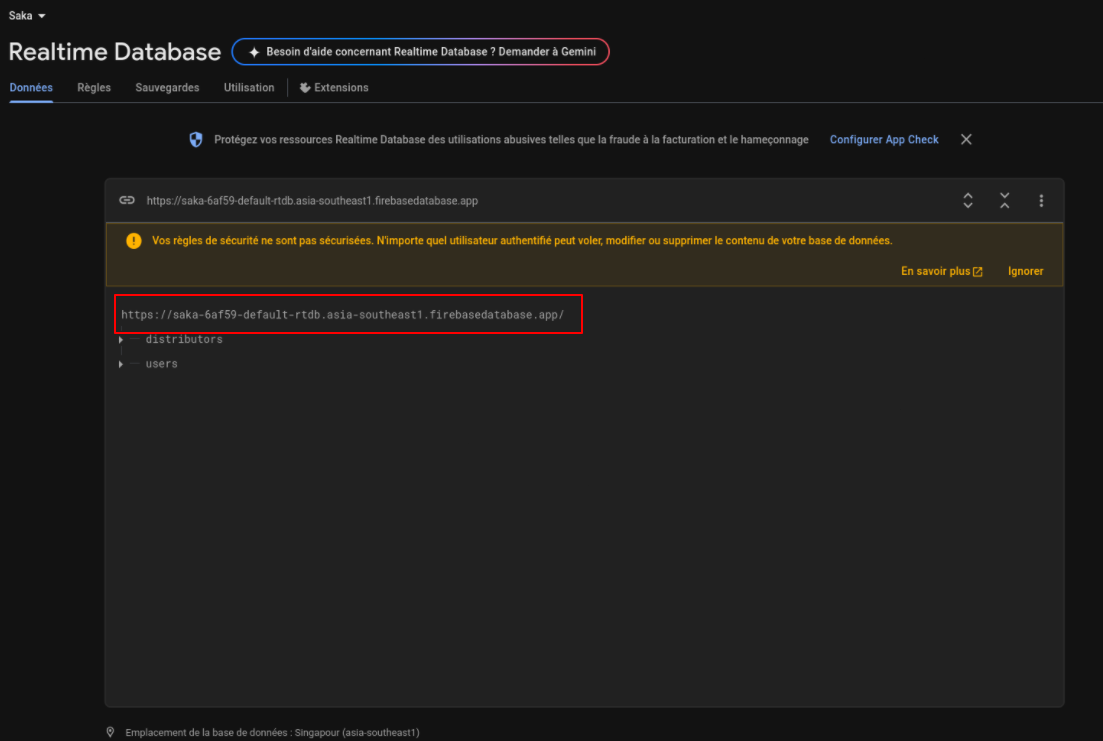
\includegraphics[scale=0.54]{firebase_realtime_db.png}
   \caption{La base de données dans Realtime Database}
   \label{fig:db_dans_realtime_db}
\end{figure}


\section{Développement de l'application mobile}
	\subsection{Repository}
		Les classes \verb|Repository| sont des classes d'abstraction de la communication vers la base de données. Elle sont appelé par la partie du code qui gère l'interface utilisateur pour récupérer les données. 	Dans la figure~\ref{fig:history-repository}, la classe \verb|HistoryRespository| permet de récupérer les données des historique de distributions. 
	\begin{figure}[H]
   			\centering
   			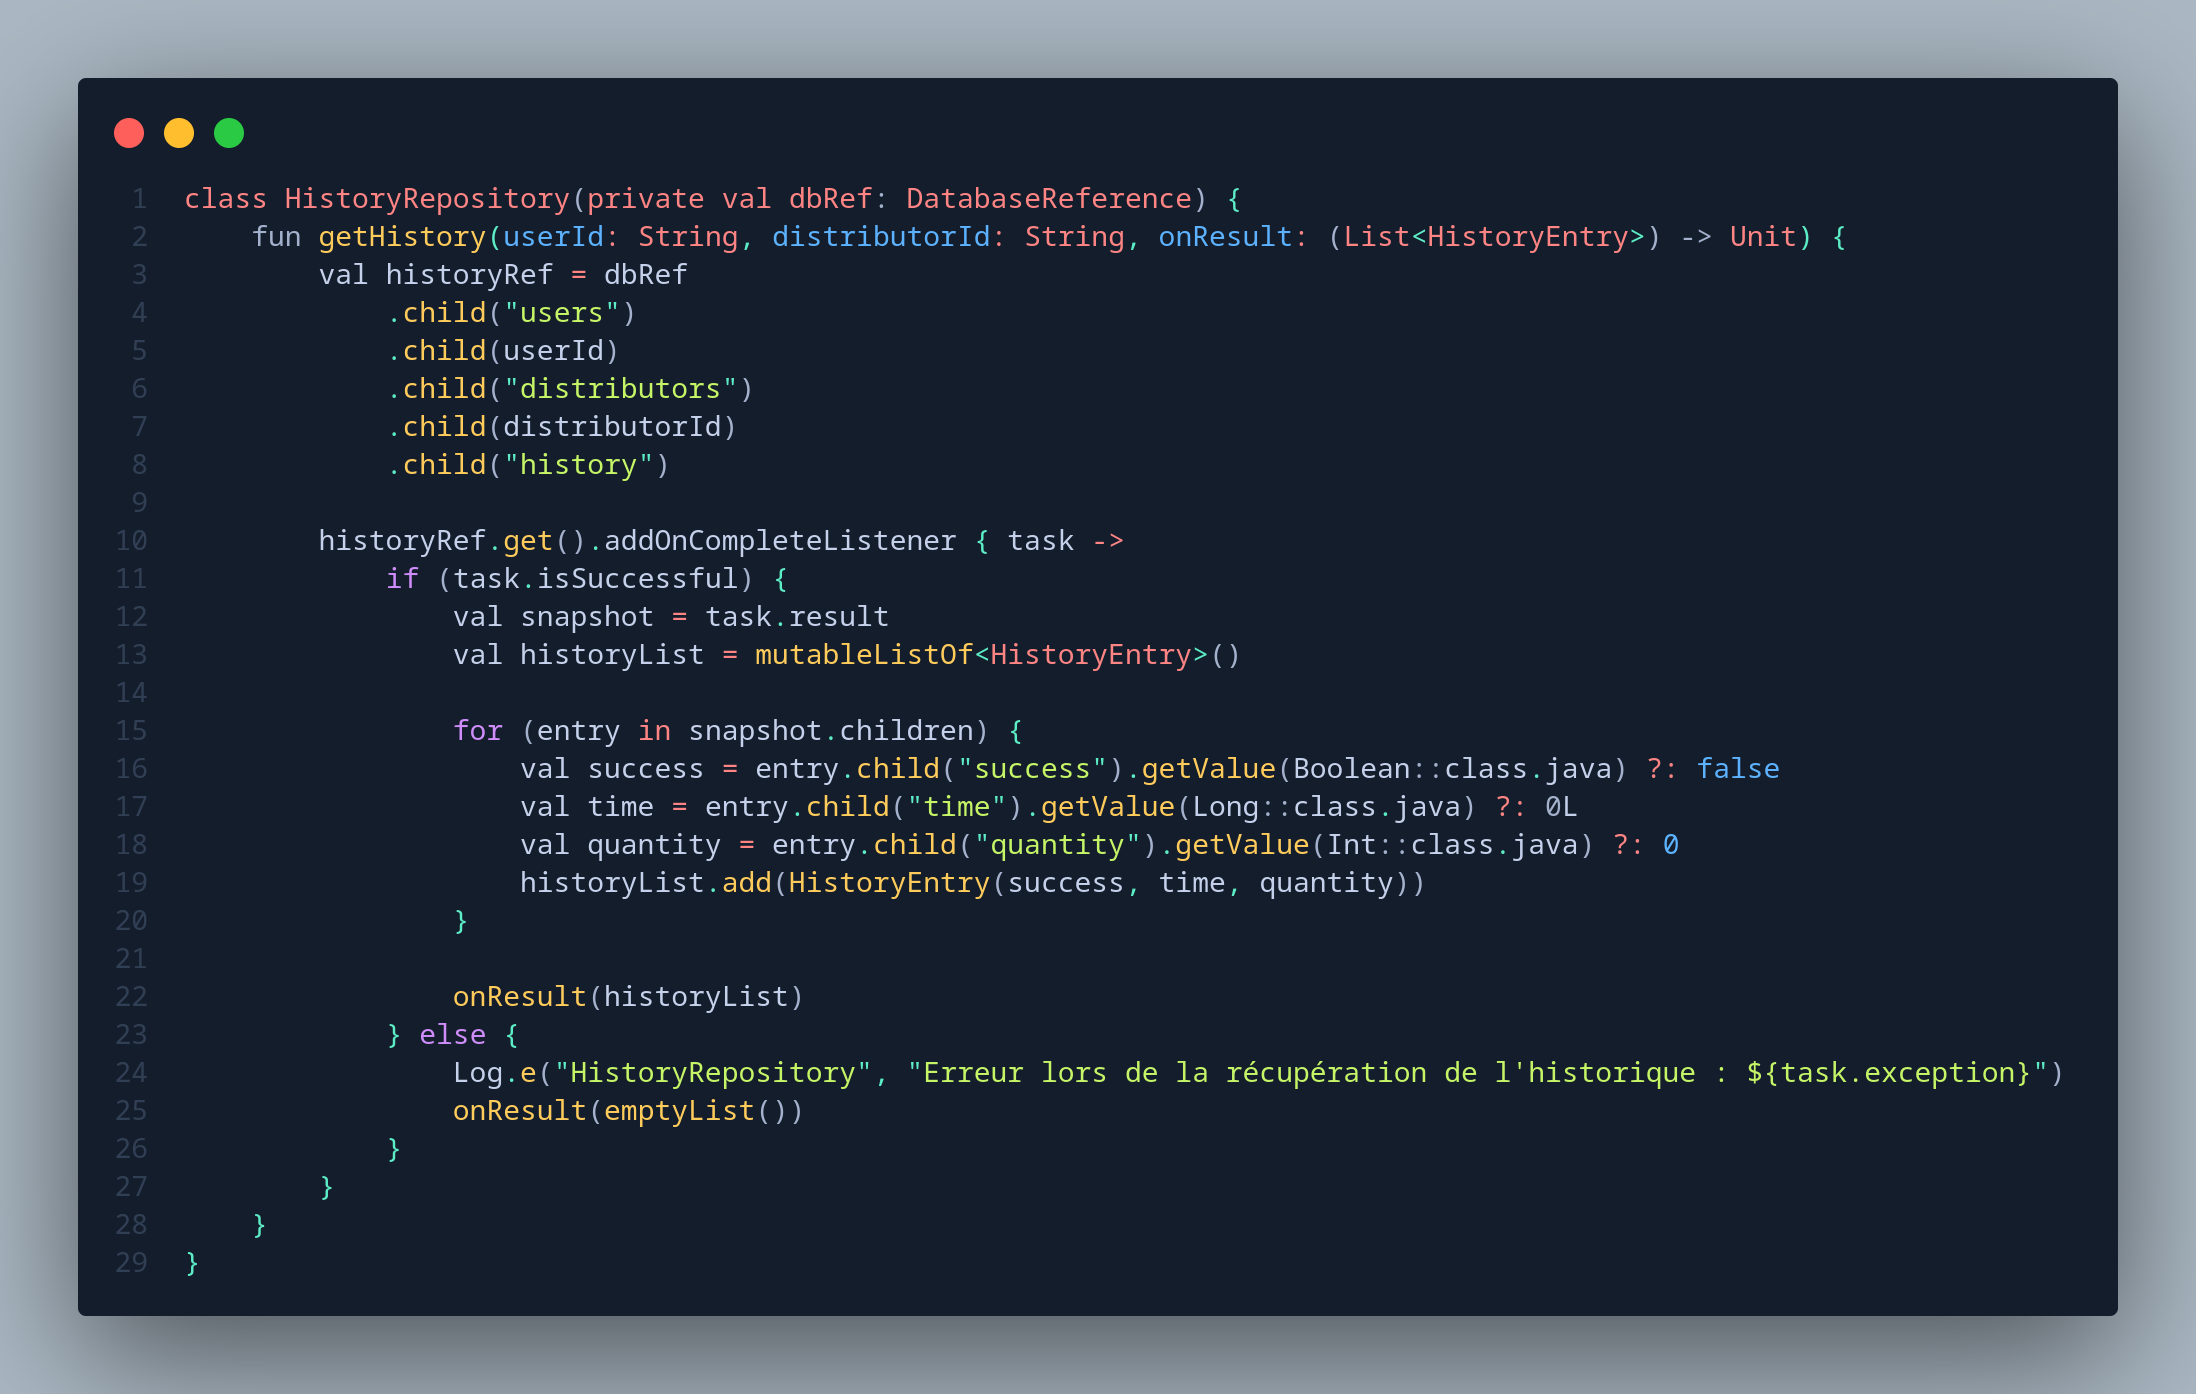
\includegraphics[scale=0.2]{history-repository.png}
   			\caption{Extrait de code d'une classe Repository}
   			\label{fig:history-repository}
	\end{figure}
	
\subsection{Interface utilisateur}
	L’interface utilisateur a été créée avec Kotlin combiné avec Jetpack Compose afin de proposer une interface conviviale, moderne et réactive.
La figure~\ref{fig:ui-code} illustre l’utilisation de Jetpack Compose pour la mise en place de l’écran d’historique. Cet extrait de code montre la structure globale de l’écran HistoryScreen, avec la gestion de l’état (par exemple, la période sélectionnée), le chargement dynamique des données depuis la base de données en arrière-plan, et l’affichage conditionnel des éléments filtrés.
On y voit également l’intégration d’un TopBar et d’un BottomNavigationBar, des filtres de période sous forme de FilterChip, ainsi que l’affichage d’une liste d’entrées via des Card, offrant une expérience utilisateur fluide et interactive.
	
	\begin{figure}[H]
   			\centering
   			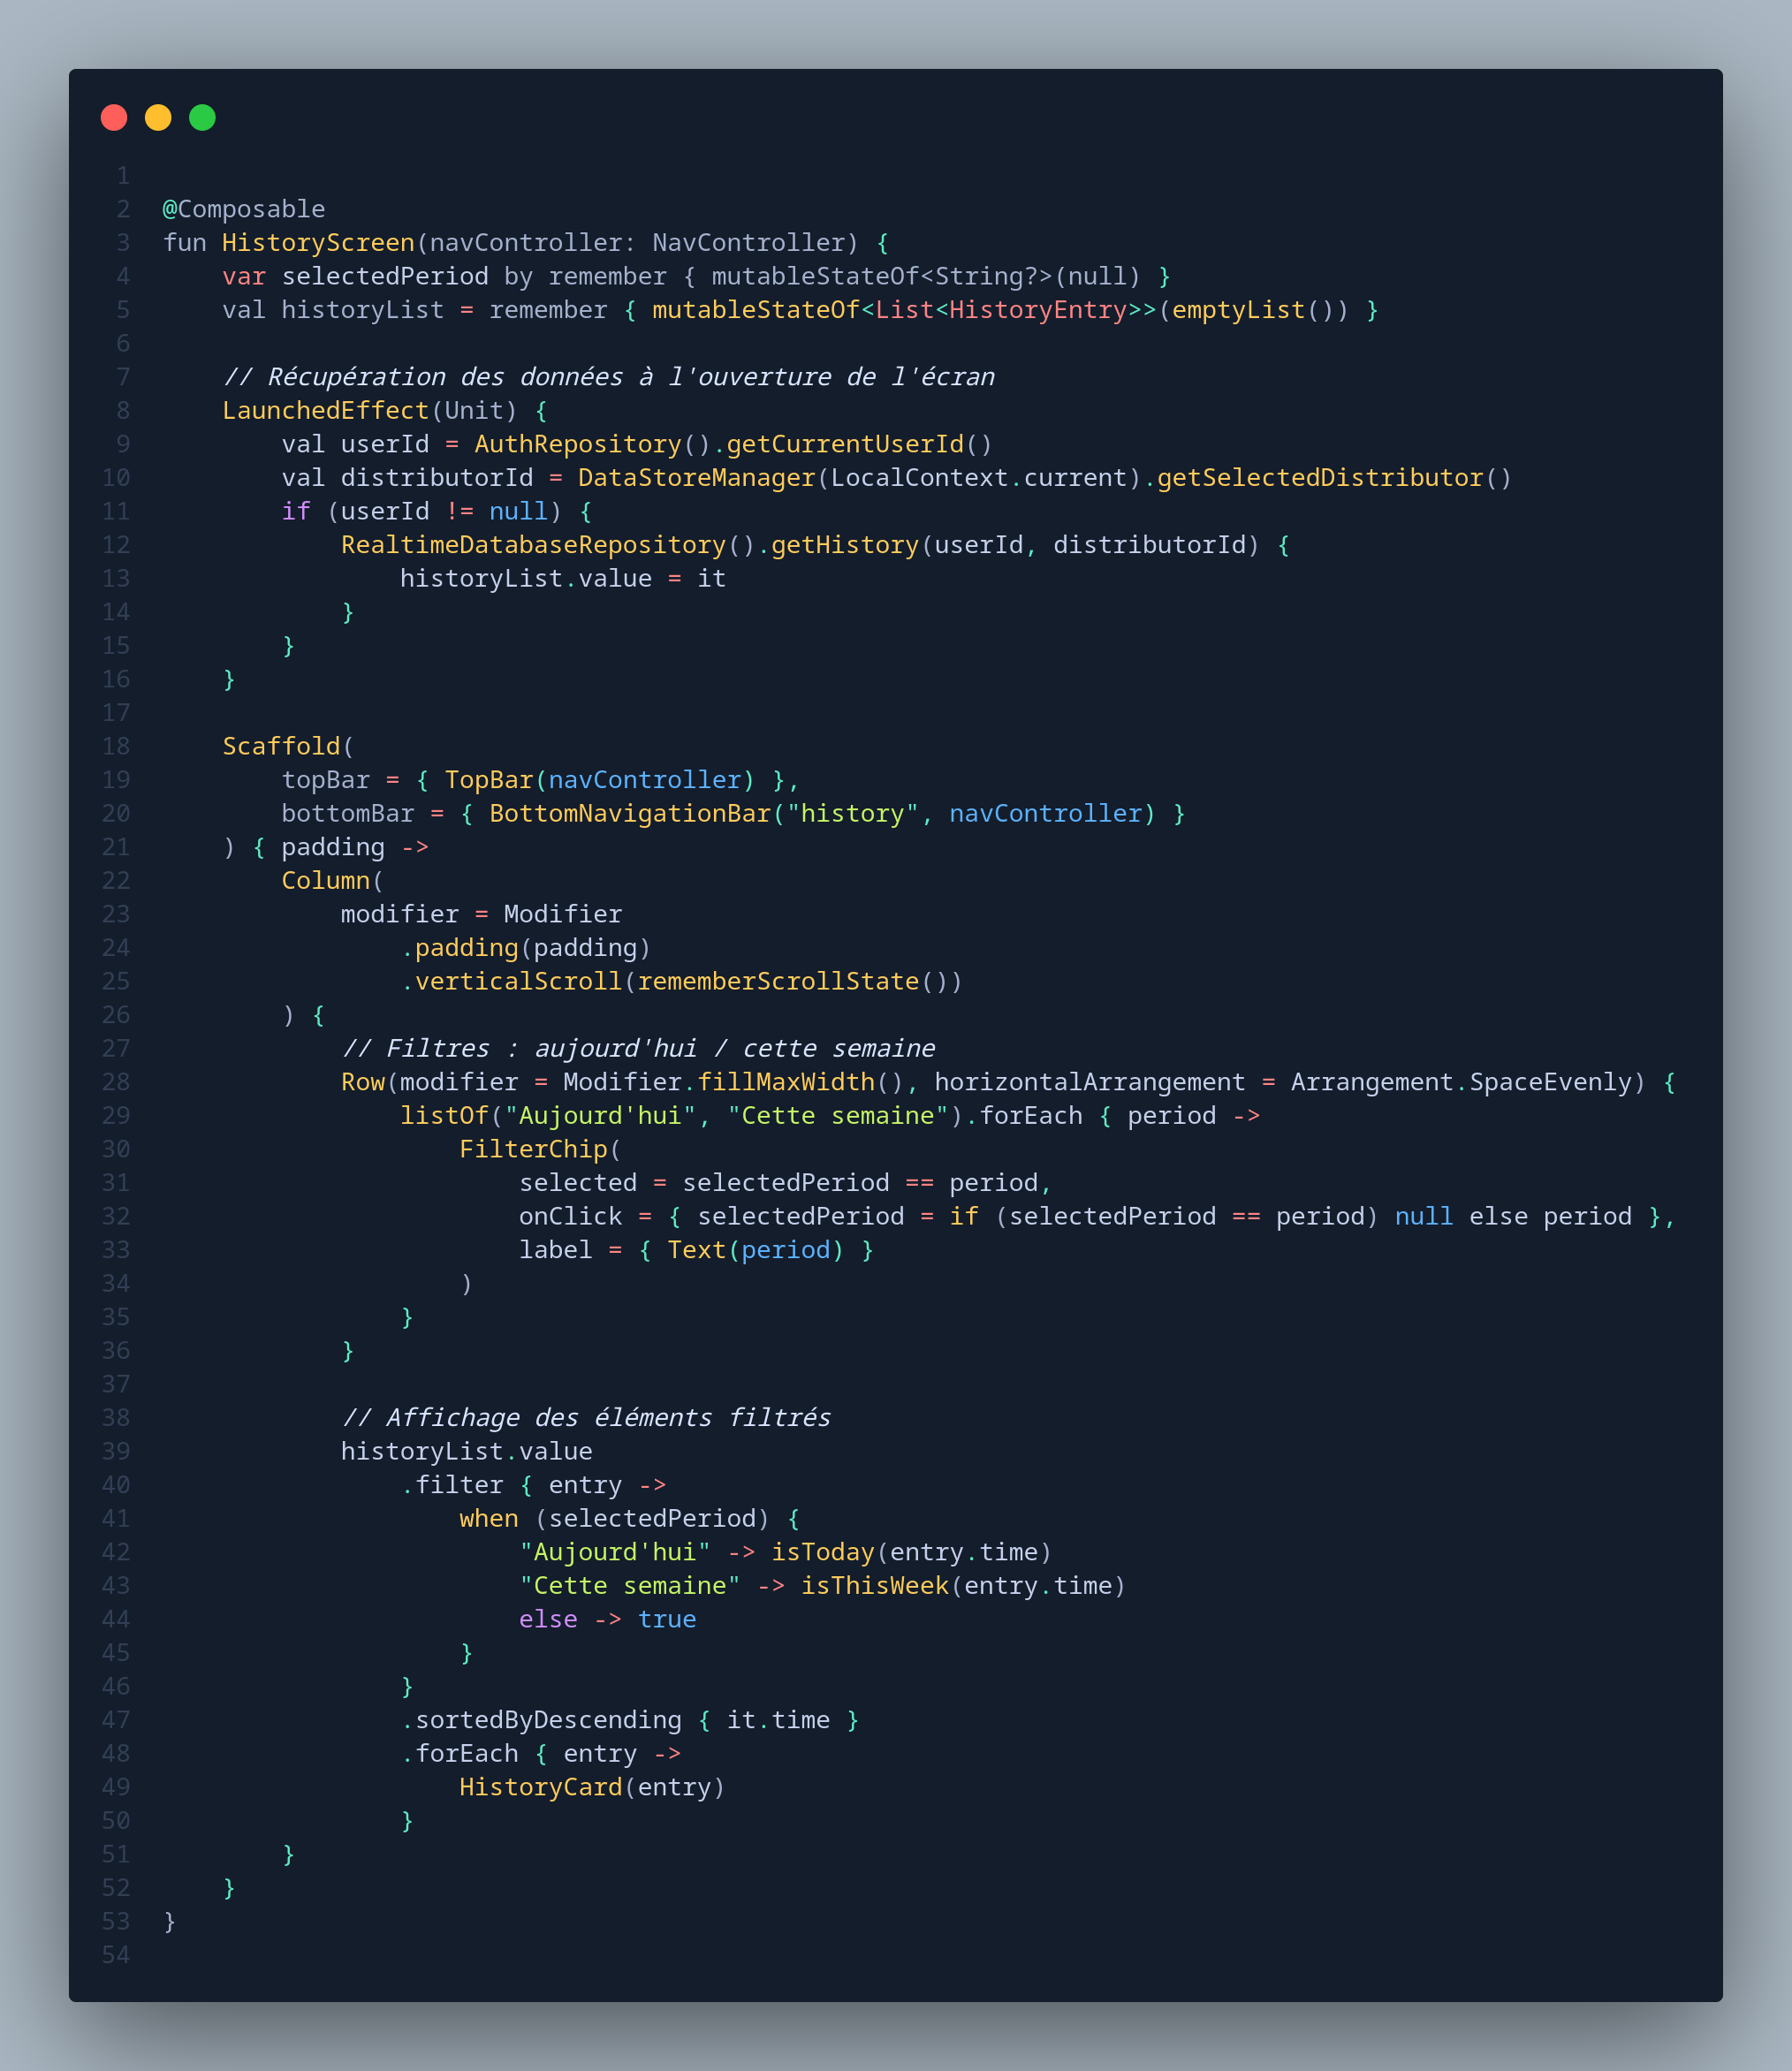
\includegraphics[scale=0.22]{ui-code.png}
   			\caption{Extrait de code de l'interface utilisateur}
   			\label{fig:ui-code}
	\end{figure}
	
\section{Développement du serveur websocket}
\subsection{Besoin}
Le serveur websocket devrait être utilisé pour : 
\begin{itemize}
\item récupération des paramètres des distributeurs dans la base de données
\item détection des déclenchements manuels 
\item surveillance de l'état de connexion de l'ESP32 à internet
\item mise en place des crons pour les distributions planifiés
\item récupération des données des capteurs et les stocker dans la base de données
\end{itemize}

\subsection{Codage du serveur WebSocket}
Les étapes suivantes ont été suivies durant le développement du serveur WebSocket :
\begin{itemize}
\item Initialisation du serveur WebSocket : la bibliothèque \textbf{express-ws} a été utilisée pour l'implémentation du serveur afin d'accélérer le développement en abstrahant la gestion manuelle des messages WebSocket. La figure~\ref{fig:express-ws} illustre comment cela est mis en place.

\begin{minipage}{\linewidth}
  \centering
  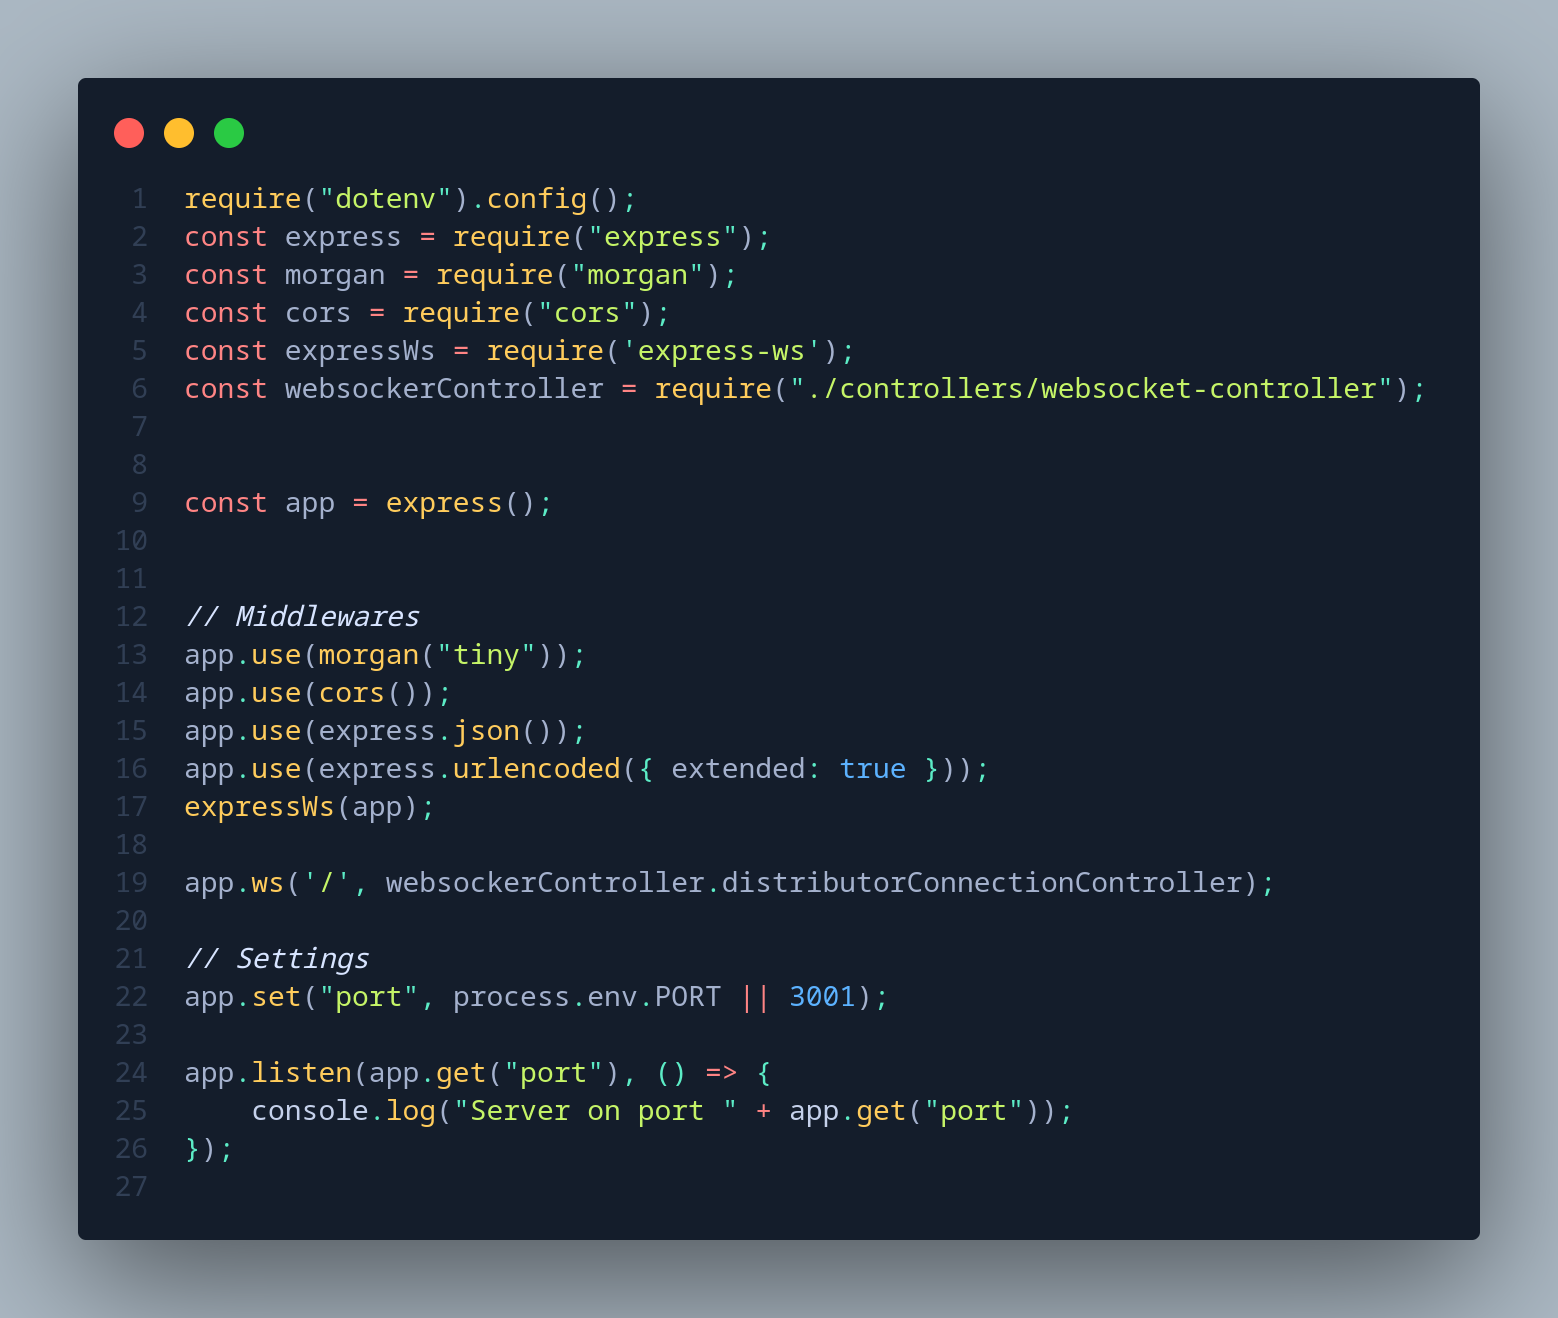
\includegraphics[scale=0.25]{express-server.png}
  \captionof{figure}{Initialisation du serveur WebSocket}
  \label{fig:express-ws}
\end{minipage}
\\

\item Initialisation de la connexion vers Firebase Realtime Database : pour cela, nous créons un compte de service dans la base de données et récupérons ses identifiants de connexion sous forme de JSON, que nous chargeons dans la variable d'environnement \verb|FIREBASE_CONFIG| afin de garantir que le code ne contient pas d'informations sensibles. La figure~\ref{fig:firebase-initialization} montre comment nous utilisons cette variable d'environnement pour initialiser la connexion vers Firebase Realtime Database.

\begin{minipage}{\linewidth}
  \centering
  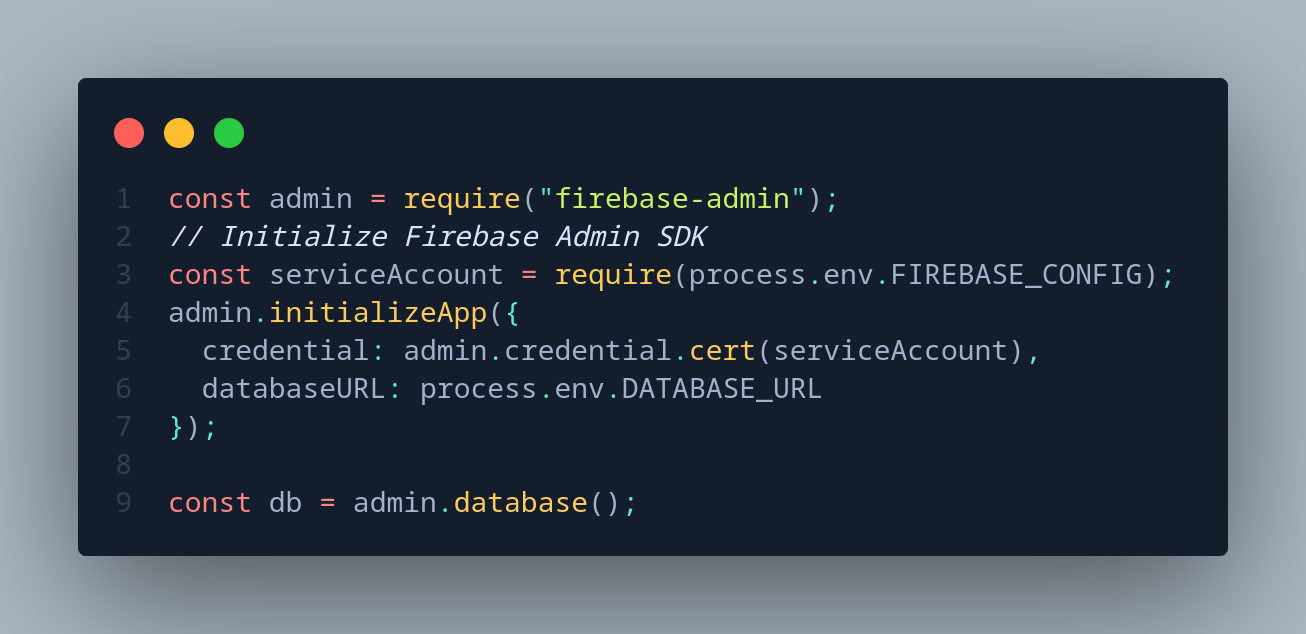
\includegraphics[scale=0.3]{firebase-initialization.png}
  \captionof{figure}{Initialisation de la connexion vers Firebase Realtime Database}
  \label{fig:firebase-initialization}
\end{minipage}
\\

\item Récupération des données : la récupération asynchrone des données se fait en ciblant la hiérarchie du JSON dans la fonction \verb|db.ref|. Ceci est illustré par l'extrait de code dans la figure~\ref{fig:recuperation-donnees}.

\begin{minipage}{\linewidth}
  \centering
  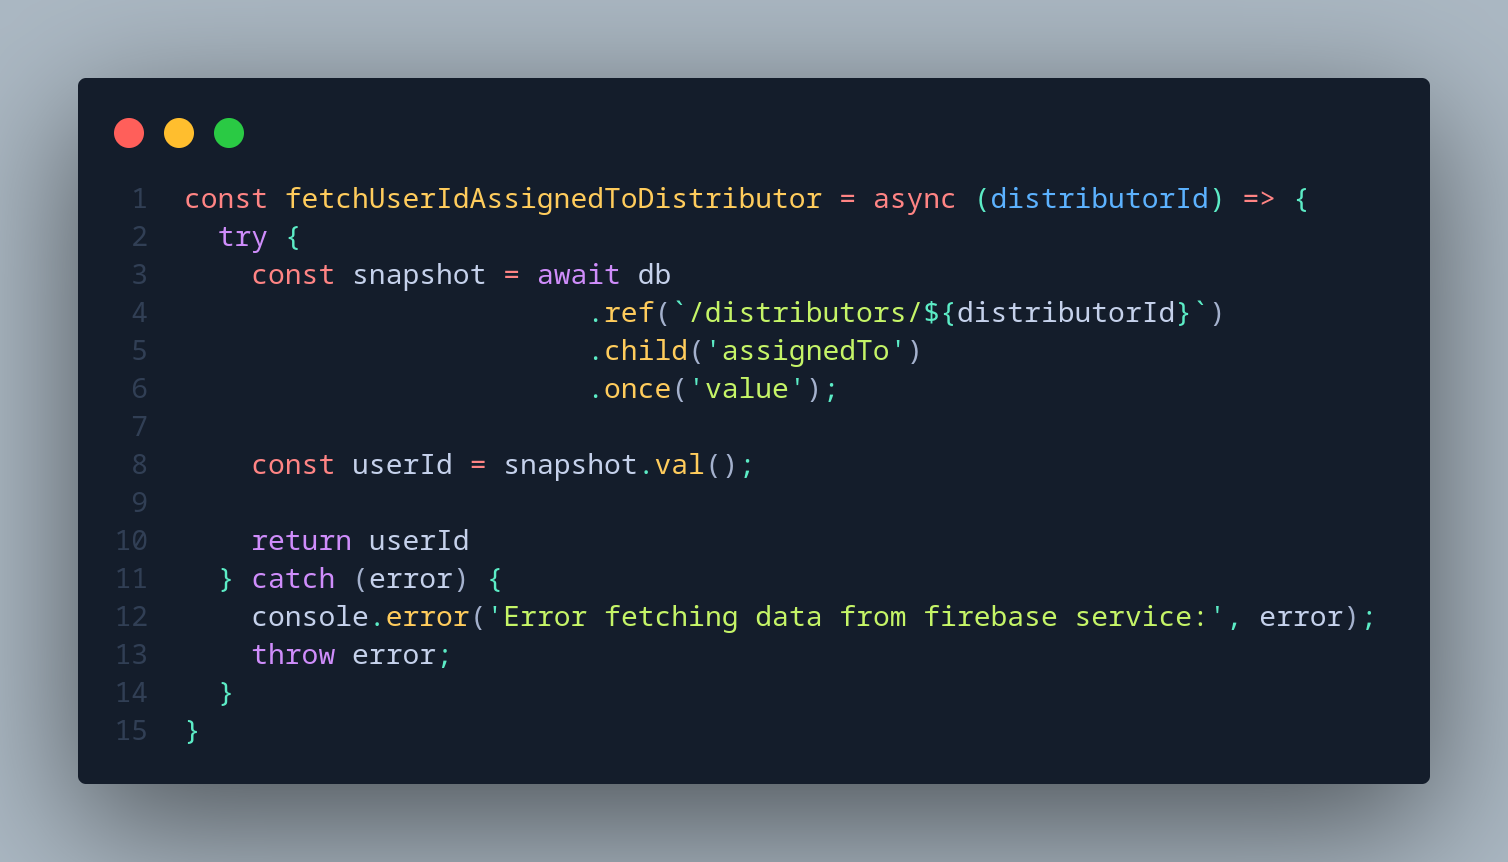
\includegraphics[scale=0.25]{recuperation-donnees.png}
  \captionof{figure}{Récupération des données}
  \label{fig:recuperation-donnees}
\end{minipage}
\\

\item Envoi des données et des commandes vers l'ESP32 : ceci se fait globalement par des messages WebSocket. On suit le format JSON pour les communications entre le serveur WebSocket et l'ESP32 :\begin{alltt}
{ "type": "<type_de_message>", "data": "<donnees_associees>" }
\end{alltt} 
Un exemple concret est montré par la figure~\ref{fig:envoi-donnees}, illustrant l'envoi des données de configuration initiale à l'ESP32.

\begin{minipage}{\linewidth}
  \centering
  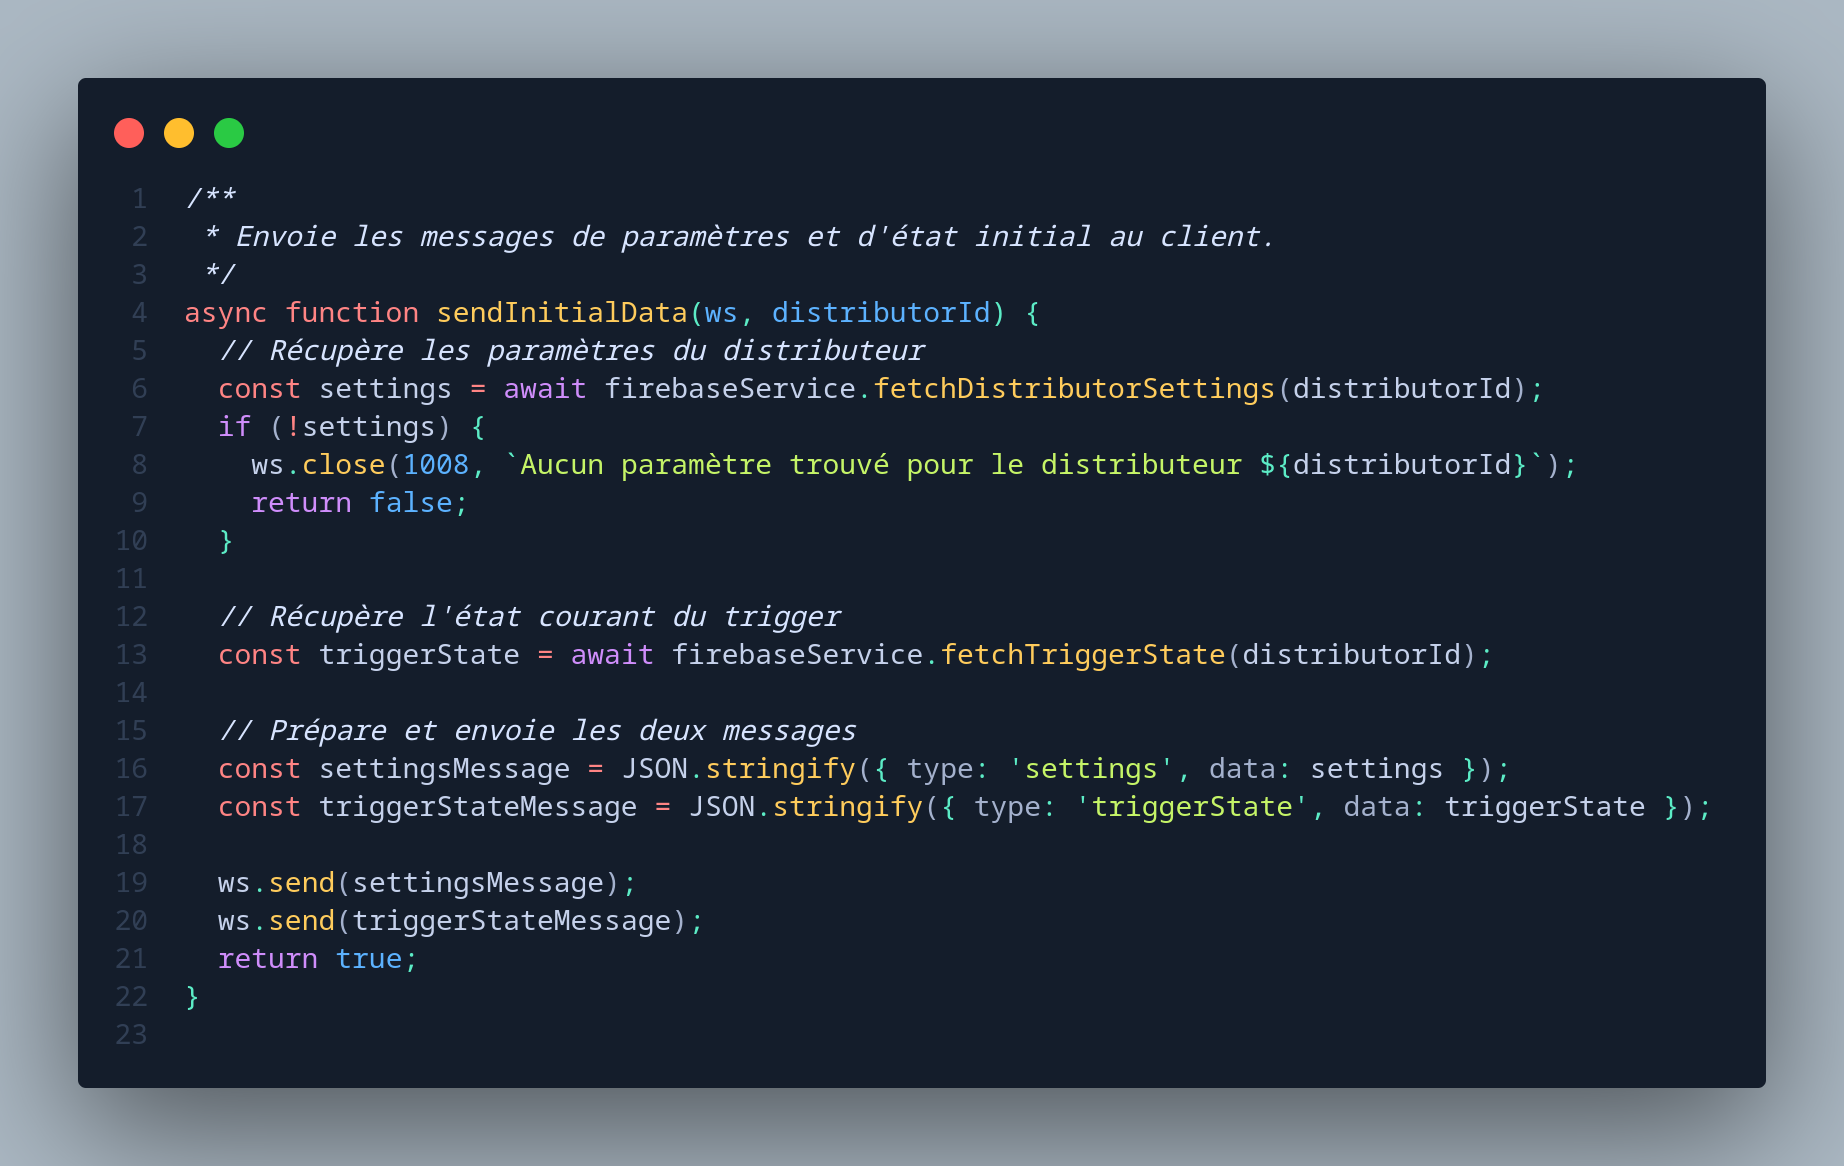
\includegraphics[scale=0.2]{envoi-donnees.png}
  \captionof{figure}{Envoi des données vers l'ESP32}
  \label{fig:envoi-donnees}
\end{minipage}
\\

\item Surveillance des changements dans la base de données : pour surveiller les changements sur une clé dans la base de données, on utilise le \textbf{Firebase Data Stream} pour surveiller en temps réel les modifications de cette clé. Le fonctionnement est simple : à chaque mise à jour des données, le serveur WebSocket est notifié de ce changement et exécute le code nécessaire. La figure~\ref{fig:surveillance-donnees} en est un exemple concret.

\begin{minipage}{\linewidth}
  \centering
  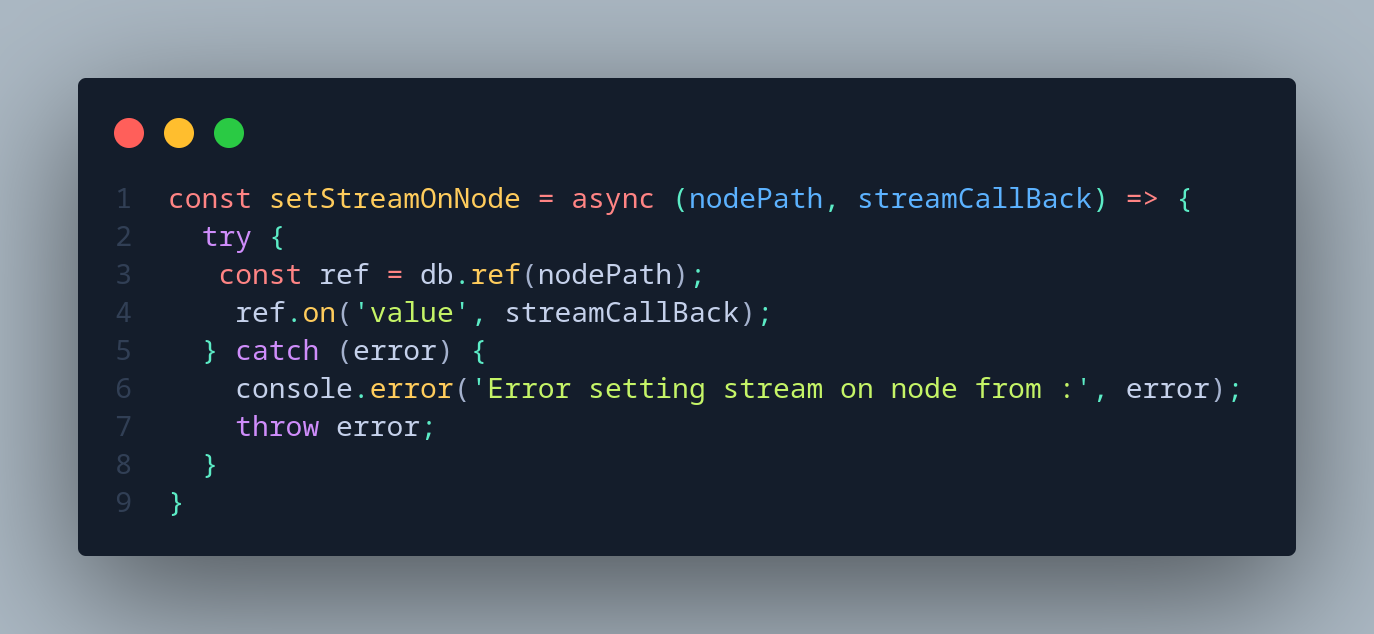
\includegraphics[scale=0.3]{surveillance-changement.png}
  \captionof{figure}{Fonction pour surveiller les changements sur une clé donnée}
  \label{fig:surveillance-donnees}
\end{minipage}
\\

\item Mise en place des scripts cron : à chaque planification détectée dans la base de données, un script cron est planifié du côté NodeJS. La figure~\ref{fig:cron-task} illustre la fonction qui prend en paramètre l'heure et l'action à exécuter pour la tâche cron associée.

\begin{minipage}{\linewidth}
  \centering
  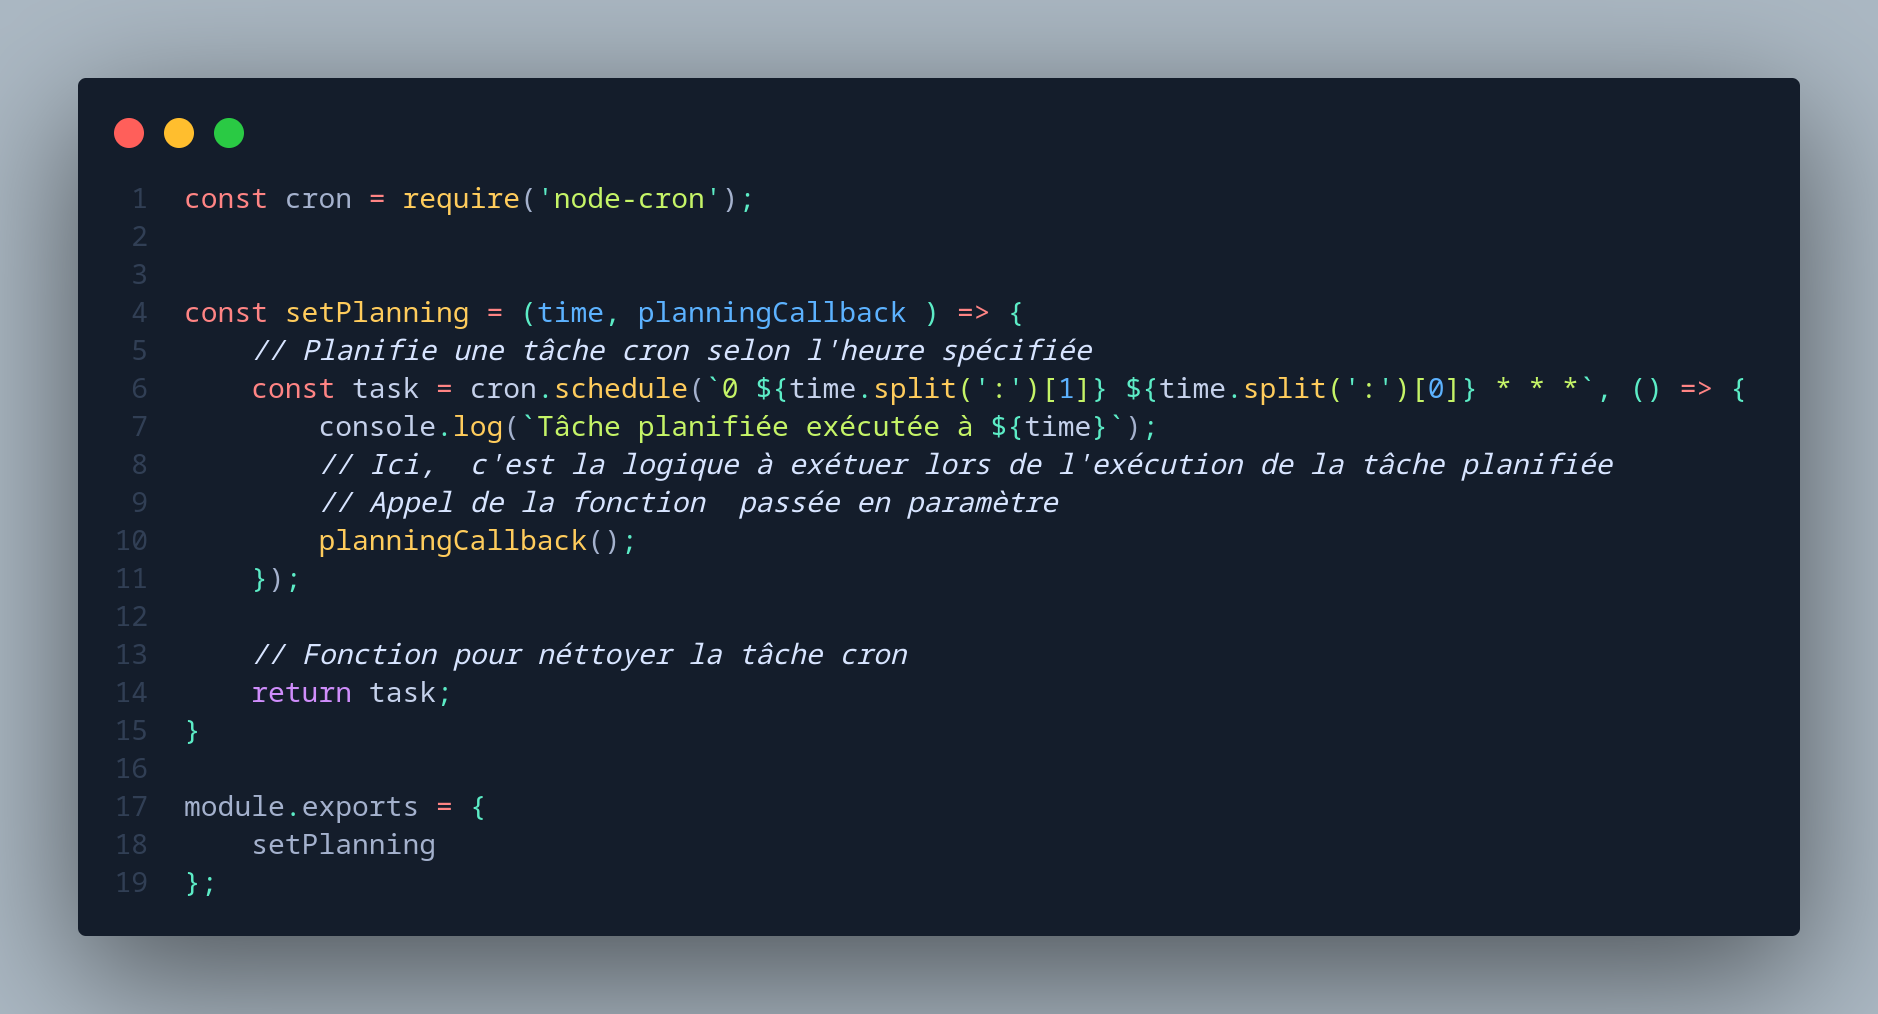
\includegraphics[scale=0.2]{cron-task.png}
  \captionof{figure}{Planification des tâches cron}
  \label{fig:cron-task}
\end{minipage}
\\
\end{itemize}


\section{Montage du système et réglages matériels}
\subsection{Capteur de pesage}
\begin{itemize}
	\item \textit{Montage} : À peine déballé, le capteur de pesage n'a aucun support attaché avec lui, d'où la nécessité de monter le support nécessaire pour le capteur. La figure~\ref{fig:montage-capteur-pesage} montre le résultat après montage des supports.
	
	\begin{minipage}{\linewidth}
  		\centering
  		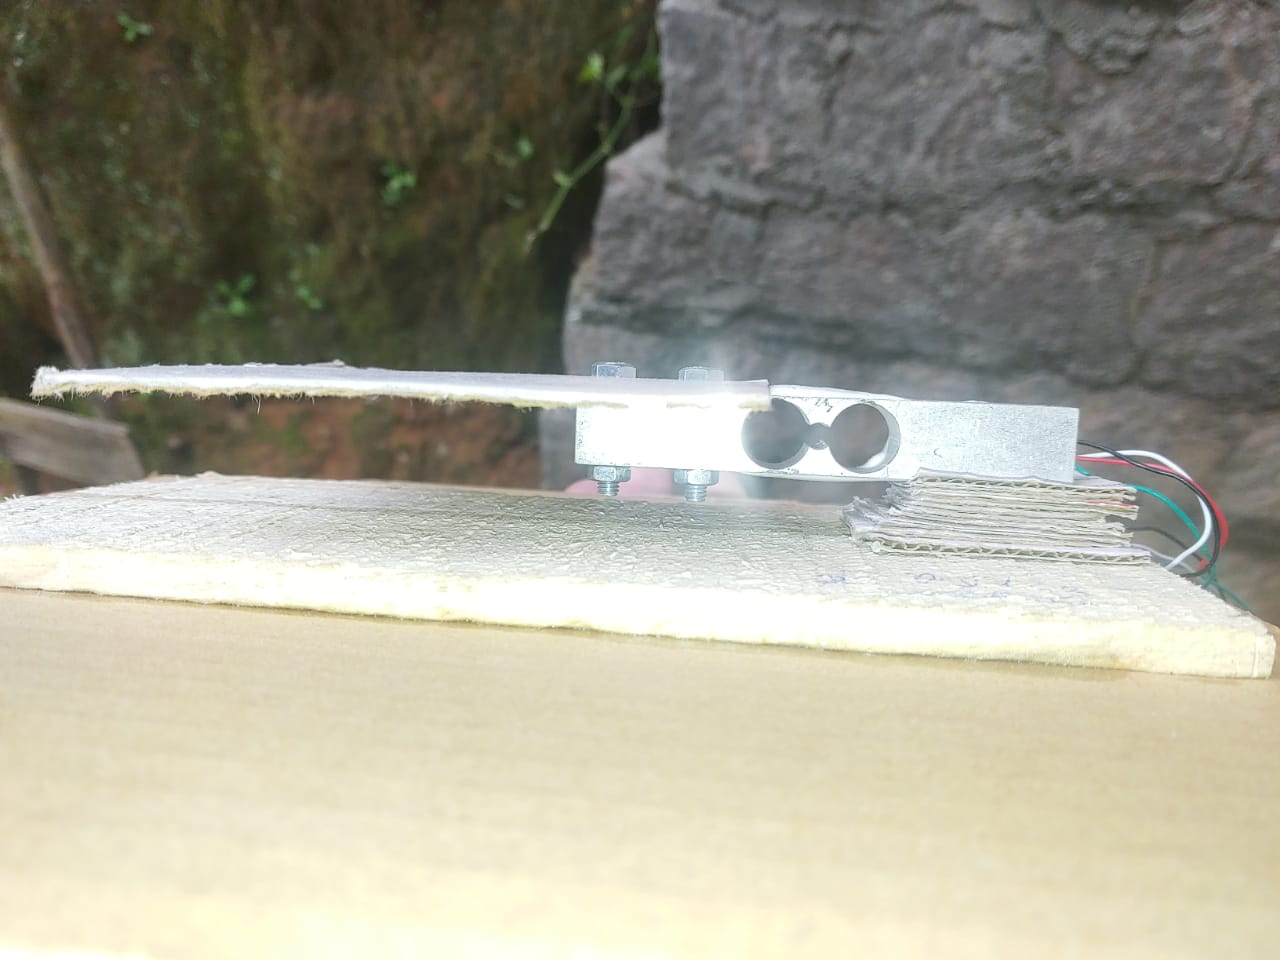
\includegraphics[scale=0.2]{montage-capteur-pesage.jpeg}
  		\captionof{figure}{Montage du capteur de pesage}
  		\label{fig:montage-capteur-pesage}
	\end{minipage}
	
	\item \textit{Calibrage} : Le calibrage se fait après le montage. Il est essentiel pour garantir la précision des mesures du capteur. Voici les étapes à suivre pour bien calibrer le capteur de pesage :

	\begin{enumerate}
		\item \textbf{Mise à zéro} : il faut s'assurez que le capteur est sans charge, puis réinitialisez la lecture à zéro pour éliminer toute valeur résiduelle.
		\item \textbf{Application d'une charge connue} : on place ensuite un poids de référence connu sur le capteur.
		\item \textbf{Lecture de la valeur mesurée} : on prend note la valeur affichée par le système de mesure.
		\item \textbf{Calcul du facteur de calibration} : on compare la valeur mesurée à la valeur réelle du poids de référence pour déterminer le facteur de calibration.
		\item \textbf{Ajustement du système} : Et enfin on entre le facteur de calibration dans le système pour corriger les futures mesures.
	\end{enumerate}

	Ce processus peut être répété avec différents poids de référence pour améliorer la précision. Il est recommandé de recalibrer régulièrement le capteur pour maintenir des mesures fiables, surtout si le capteur est utilisé fréquemment ou dans des conditions variables.
\end{itemize}


\subsection{Servo moteur}
\begin{itemize}
	\item \textit{Montage} : Un carton est fixé sur l'axe de rotation du servo moteur afin de permettre le blocage et l'ouverture de l'orifice du réservoir. Ensuite, l'ensemble est attaché au support relié au capteur de poids, comme illustré à la figure~\ref{fig:servo-moteur}.
	
	\begin{minipage}{\linewidth}
  		\centering
  		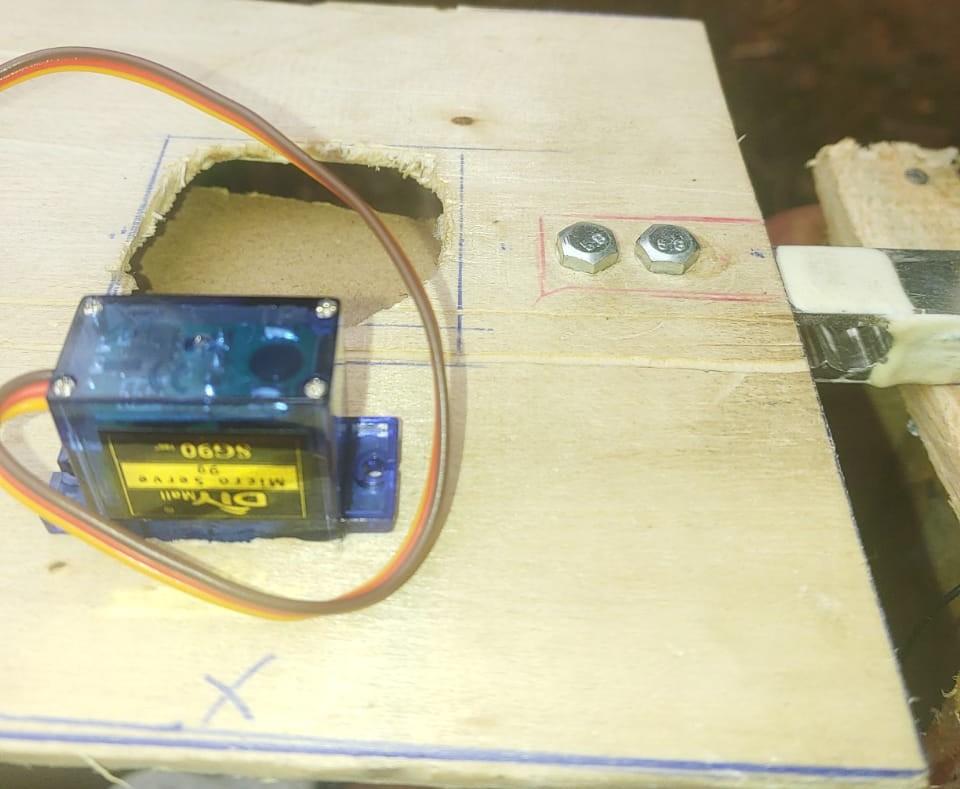
\includegraphics[scale=0.4]{servo-moteur.jpeg}
  		\captionof{figure}{Montage du servo moteur}
  		\label{fig:servo-moteur}
	\end{minipage}
	\\
	\item \textit{Configuration initiale nécessaire} :Avant la mise en service, il est nécessaire de réaliser certaines étapes de configuration afin de garantir le bon fonctionnement du servo moteur, comme illustré par l'extrait de code de la figure~\ref{fig:servo-moteur-code}.
	\begin{itemize}
		\item \textbf{Positionnement initial} : Il faut positionner le servo moteur à sa position neutre (généralement 90°) avant de le fixer mécaniquement, afin d'assurer un alignement correct.
		\item \textbf{Paramétrage du signal de commande} : Le servo moteur doit être contrôlé par un signal PWM approprié. Il convient de s'assurer que la fréquence et l'amplitude du signal sont compatibles avec les spécifications du servo utilisé.
		\item \textbf{Définition des limites de mouvement} : Les positions minimale et maximale du servo doivent être définies pour éviter tout dépassement mécanique. Cela permet de prévenir les surcharges et d'assurer une longévité accrue du dispositif.
		\item \textbf{Tests de fonctionnement} : Après configuration, des tests doivent être effectués pour vérifier que le servo moteur répond correctement aux commandes et que le mécanisme associé fonctionne comme prévu.
	\end{itemize}
	
	\begin{minipage}{\linewidth}
  		\centering
  		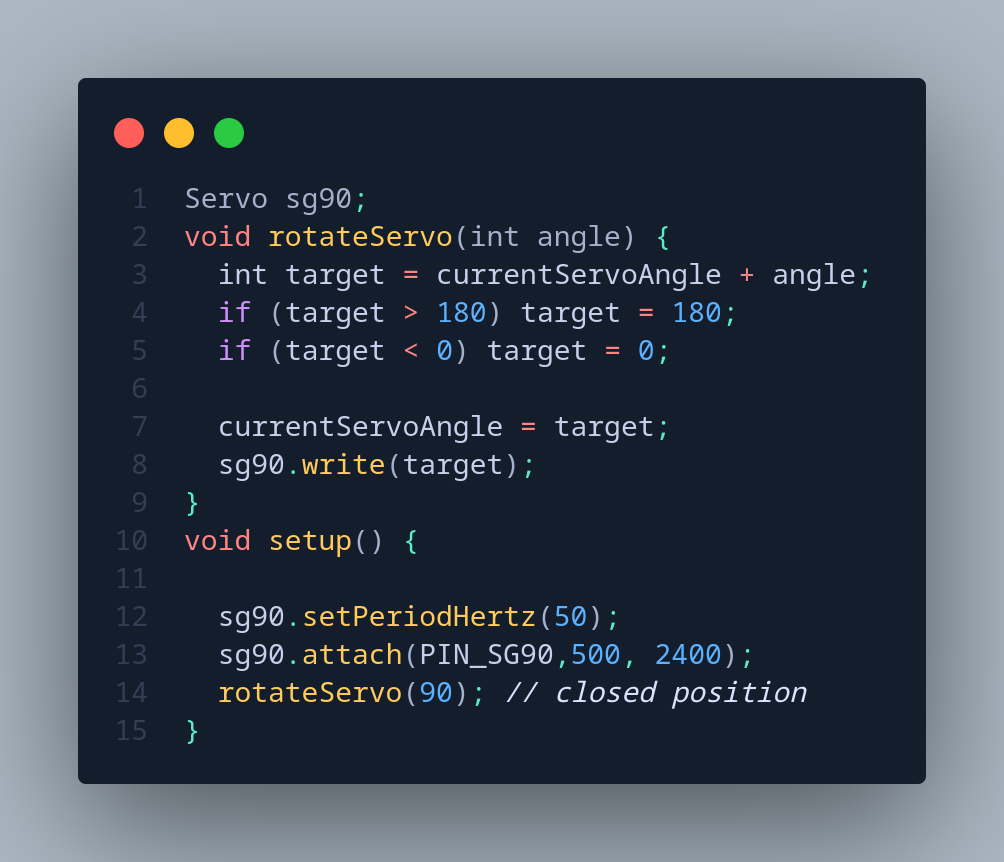
\includegraphics[scale=0.4]{servo-moteur.png}
  		\captionof{figure}{Extrait de code pour le servo moteur SG90}
  		\label{fig:servo-moteur-code}
	\end{minipage}
\end{itemize}


\subsection{ESP32}
\begin{itemize}
	\item Connexion au wifi et au serveur websocket : la figure~\ref{fig:wifi-websocket} illustre comment on établit d’abord la connexion au réseau wifi, puis comment on initialise la connexion avec le serveur websocket. Ces étapes sont indispensables pour assurer une communication stable entre l’ESP32 et le serveur.
	
	\begin{minipage}{\linewidth}
  		\centering
  		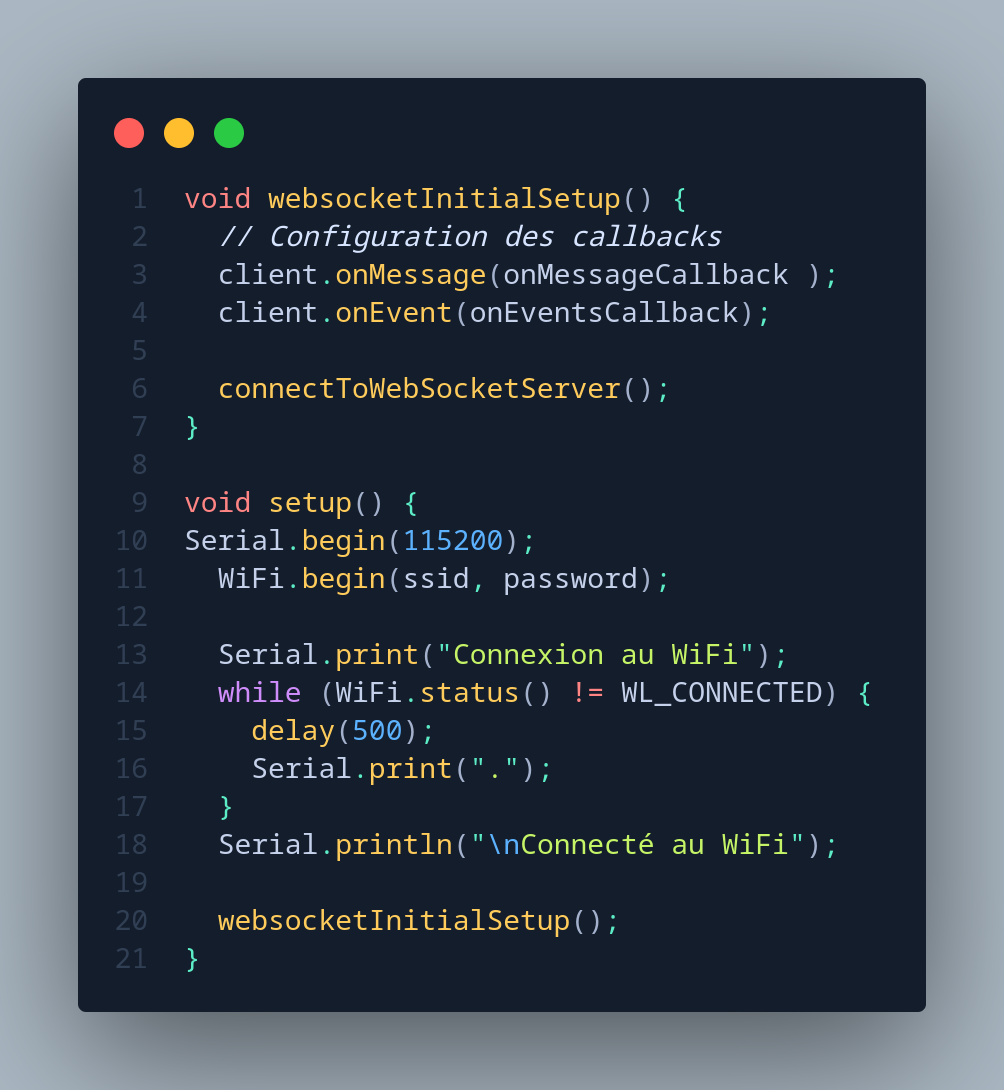
\includegraphics[scale=0.4]{wifi-websocket.png}
  		\captionof{figure}{Connexion Wifi et Initialisation du Serveur Websocket}
  		\label{fig:wifi-websocket}
	\end{minipage}
	\\
	
	\item Gestion des messages depuis le serveur websocket :la figure~\ref{fig:message-websocket} montre comment on récupère un message JSON, on extrait le type et les données, puis on effectue des actions spécifiques selon le type reçu (comme faire bouger le servo ou envoyer une réponse au serveur).\\
	\begin{minipage}{\linewidth}
  		\centering
  		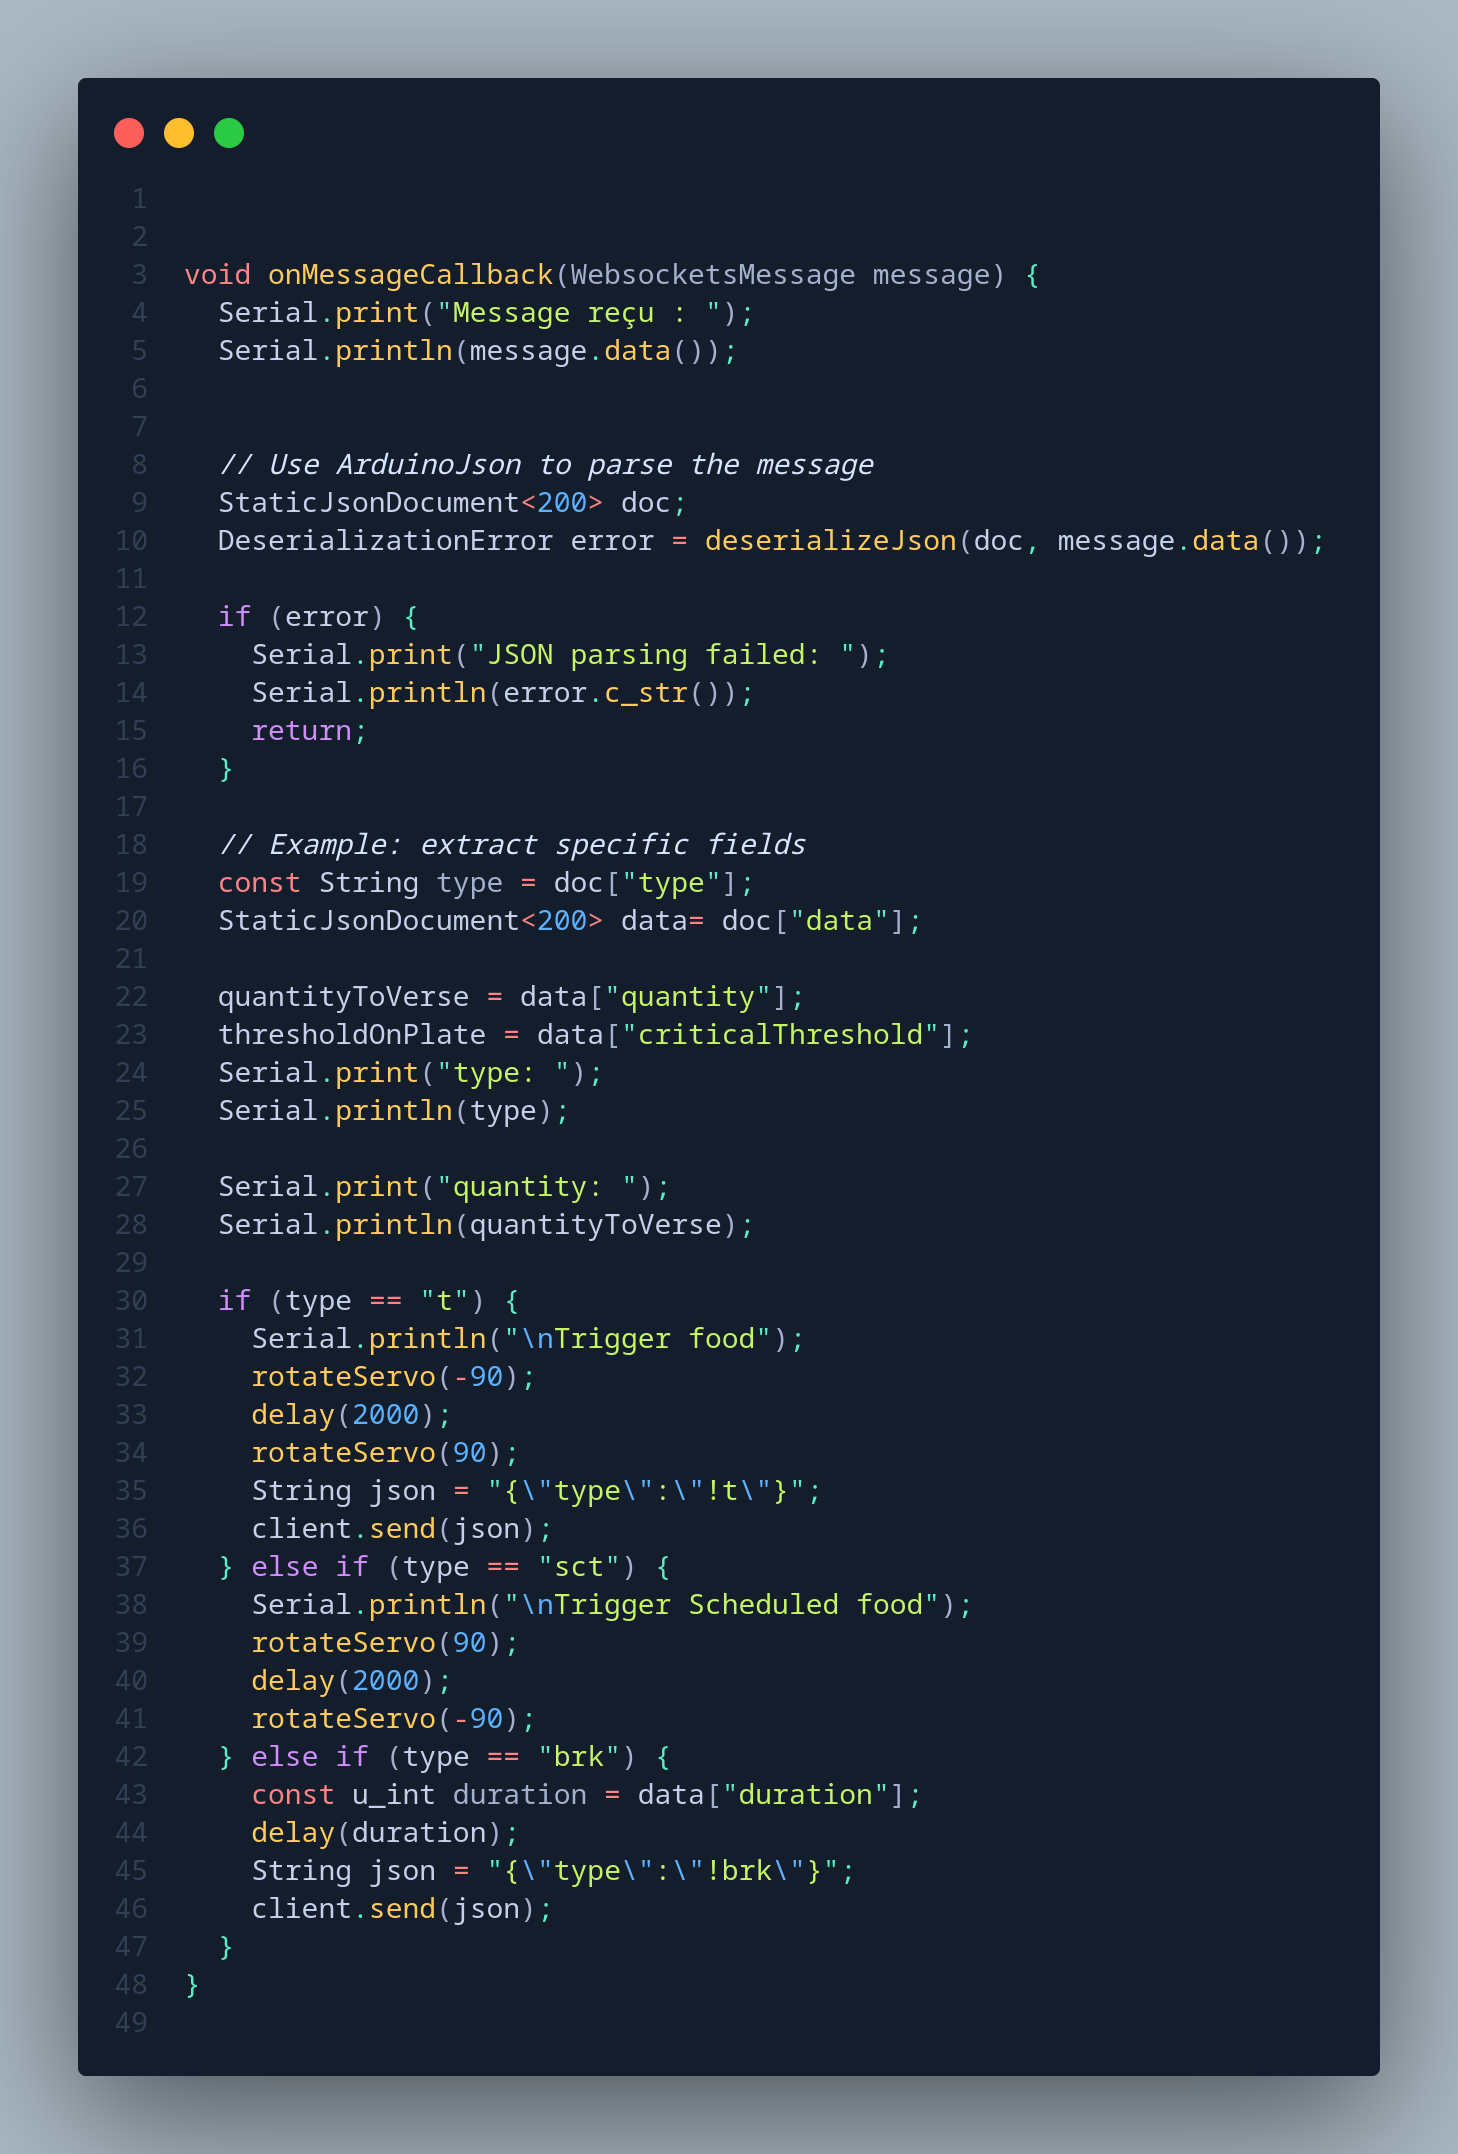
\includegraphics[scale=0.3]{message-websocket.png	}
  		\captionof{figure}{Réception et Gestion des Messages depuis le Serveur Websocket}
  		\label{fig:message-websocket}
	\end{minipage}
\end{itemize}


